%!TEX root = ../report.tex

\section{Public Key Infrastructures (PKI)}
A PKI is an infrastructure that handles certificates in a untrusted network.
Certificates are cryptographic bindings between an identifier and a public key that is to be associated with that identifier.
The identifier often refers to persons or businesses, but can also be other attributes like access rights.
What is always necessary is that it has to be verified that the identifier and corresponding key belong together.
In case of persons or businesses, additionally a verification that the entity behind the name is the entity it claims to be.\\

PKIs are created by issuing certificates between entities.
An certificate issuer, which is a trusted third party and whose certificate and thus public key ($K_{I-pub}$) we know, creates a signature for a third party $X$ and its public key $K_{X-pub}$ with its private key $K_{I-priv}$.
The tuple of $(X,K_{X-pub},Sig_{K_{I-priv}(X|K_{X-pub})})$ is then called a certificate.
In reality, other attributes are stored in certificates additionally.\\

PKIs can either be hierarchical or not.
In hierarchical PKIs the issuers are often called certificate authorities (CA), in non-hierarchical ones endorsers.
The first mentioned type here has one central CA.
This is problematic though because who is to decide that the CA is trustworthy (In reality this trust management is done by operating systems or browsers).
Furthermore there is a high load on the CA which can lead to sloppy work which results in mistakenly issued certificates.
In some cases hierarchical CAs have intermediate registration authorities (RA) that do the verification step of identifying $X$ but do not issue certificates.
But this does not resolve the problem that there still is only one CA but merely reduces its workload.
The solution for this used in reality is to have multiple CAs which represent different legislations and which are all accepted equally.
This may increase the danger that one fucks up though.
\\
In non-hierarchical PKIs every participant can issue certificates.
Different trust metrics are used to automatically reason about authenticity of the bindings between entity and key like defining rules for how many levels of indirections are allowed.

\subsection{X.509}
X.509 is the certificate standard used in SSL/TSL and thus in a large part of the Internet.
\begin{figure}[h]
  \begin{minipage}{.49\textwidth}
    \centering
    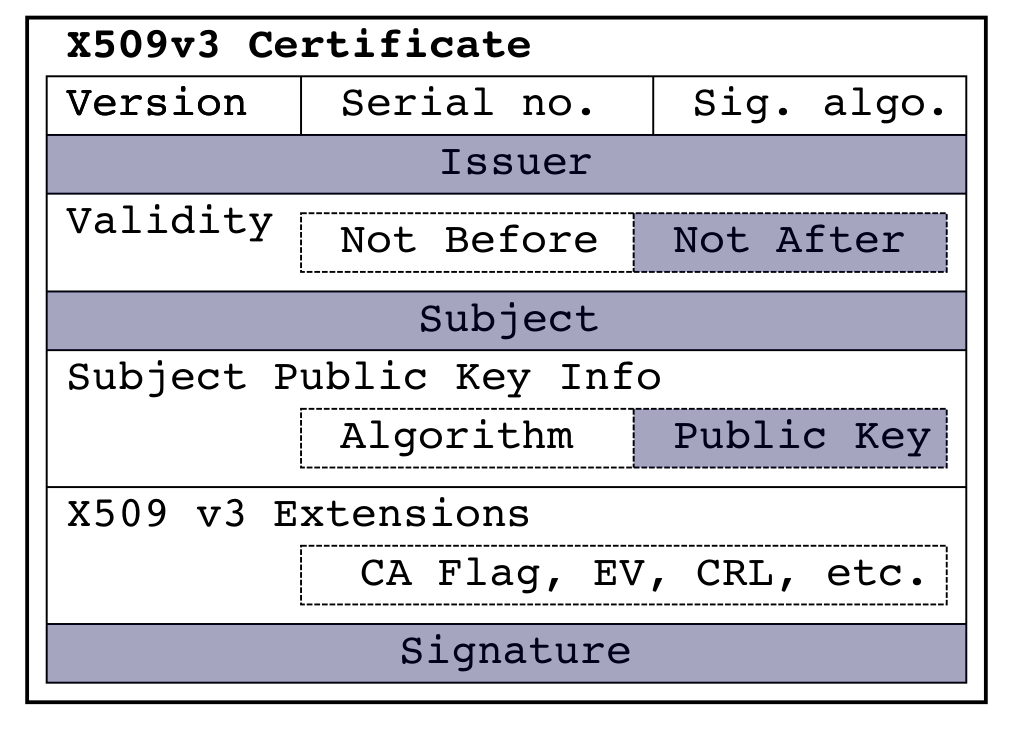
\includegraphics[width=\textwidth]{figures/x509_certificate.png}
    \caption{X.509 Certificate}\label{fig:x509_certificate}
  \end{minipage}
  \begin{minipage}{.49\textwidth}
    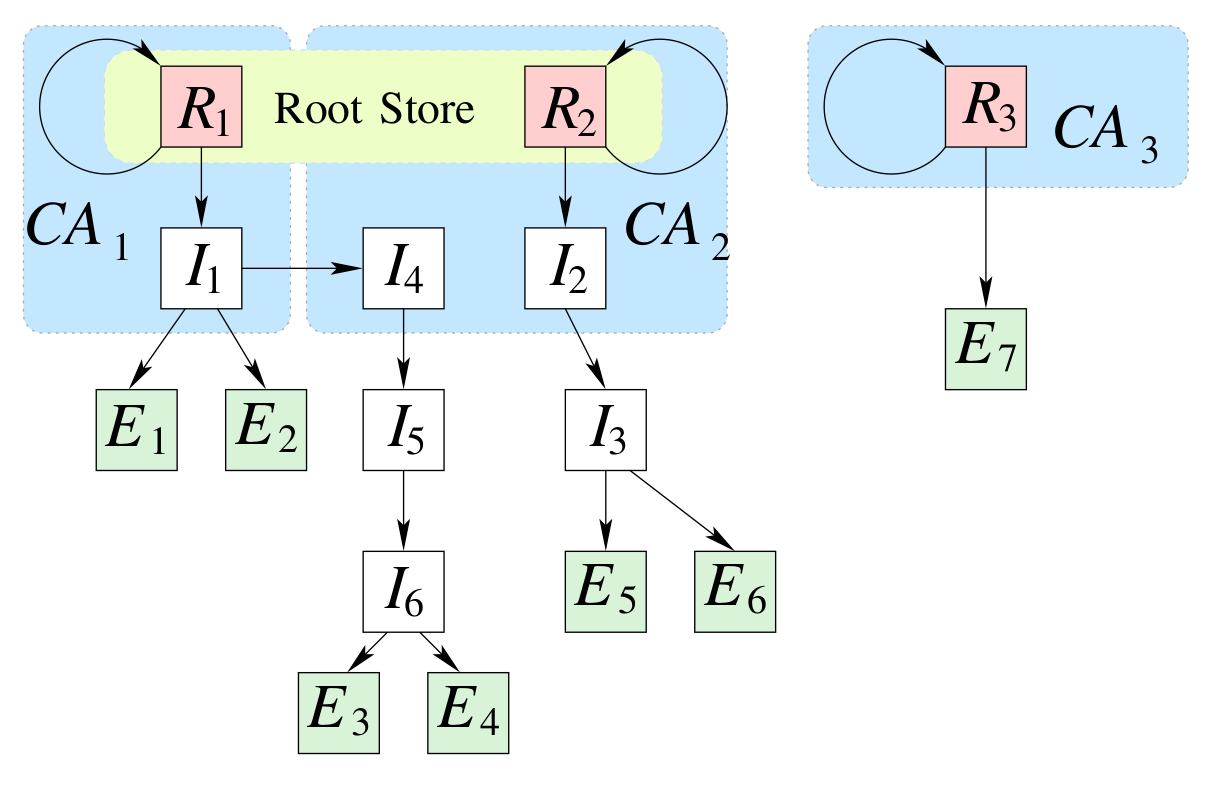
\includegraphics[width=\textwidth]{figures/x509_root_store.png}
    \caption{X.509 Root Stores}\label{fig:x509_root_store}
  \end{minipage}
\end{figure}
It relies an root stores which contain certificates of trusted CAs.
These root stores are usually managed by the operating system or the browser.
Root store certificates then usually are used to sign intermediate certificates first instead of actual host certificates because this way root certificates can be protected and signing can be delegated to sub-CAs.
A special form of this is cross signing where CAs sign a certificate of other CAs.
This undermines the trust chain of the Internet though.

\subsubsection{Certificate Issuance}
Certificates are either validated with domain validation (DV) or an Extended Validation (EV).
In DV, one has to send an e-mail to the chosen CA with information about the domain (whois details, DNS txt record, address is well known contact of the domain, \dots).
The ownership of the e-mail address thereby validates the ownership of the domain.
In EV, strong legal documents are required to prove identities.\\
Also approaches that lay in between are possible.

\subsubsection{Certificate Revocation}
Certificates have to be valid at the time of interest (e.g.\ a site is requested)and has therefore to be proven for revocation at that point.
This can be done in several ways.

The first approach are \textbf{Certificate Revocation Lists (CRL)} which are lists of revoked certificates issued, maintained and updated by CAs.
Browsers then should download these lists every time an CRL is updated and check for revoked certificates on site requests.
In reality CRLs are barely used since time intervals between CRL updates where the system is vulnerable, the updates can be blocked by MITM and CRL can grow quite large.\\

Another approach is the \textbf{Online Certificate Status Protocol (OCSP)} where CRL-like data structures are maintained on the server-side.
In practise, every time a TLS handshake is done (not every request, inperformant), a request is sent to these servers asking if a certificate is revoked (possible answers: good, revoked, unknown).
The approach of not sending OCSP requests for every site request but bundling them together (in the TLS handshake) is called OCSP stapling.\\

Some other approaches for certificate revocation are in-browser revocation lists which maintain revoked certificates for the most important sites or short-lived certs.

\subsubsection{Pinning/TOFU}
A suggestion to enhance X.509 is to use pinning/trust on first use (TOFU).
The idea is that hosts send information about themselves on first contact (e.g.\ public key) which clients then store for later identification if they decide to trust the host.
This pinning can be static, i.e.\ there are preloaded pins provided by the Chrome or Firefox, or dynamic, i.e.\ helpful information is communicated to aid clients with pinning.\\
This concept cannot be applied for certain users though, for example citizens of an authoritarian country.
Also servers might update their keys, which might look random to clients which results in them not trusting the host and browsers cannot come with preloaded keys for all sites and keep them up to date.

\subsubsection{Public Log Schemes}
The idea behind public logs is to store some information about how issues certificates to who.
They are neutral, signed and append-only lists of certifications.\\

In X.509 the log scheme is called Certificate Transparency (CT).
